\documentclass{article}
\usepackage[
backend=biber,
style=alphabetic,
sorting=ynt
]{biblatex}
\usepackage{geometry}
 \geometry{
 a4paper,
 total={170mm,257mm},
 left=20mm,
 top=20mm,
 }
\usepackage[french]{babel}
\usepackage{optidef}
\usepackage[T1]{fontenc}




\title{\textbf{CTF FACILE}\\ \textbf{Walkthrough}}


\author{Groupe 4}
\date{5 Novembre 2021}

\begin{document}

\maketitle

\section*{Introduction}
Dans ce CTF nous verrons une des failles web connue du monde entier mais aussi une des plus répandu selon l'OWASP qui la classe à la troisième place sur dix dans son rapport 2021, il s'agit de l'injection SQL. Nous verrons aussi les dégâts engendrés par l'utilisation d'un même mot de passe pour différents comptes.
\section{NMAP}
Comme dans tout CTF, une des premières choses à faire est de découvrir les ports qui sont ouverts sur une machine et les services que celle-ci héberge. Pour cela on peut utiliser l'outil \textit{nmap}. Avec un simple scan on découvre que les ports 80 et 22 sont ouverts sur la machine. 
Sur le port 80 nous avons un serveur HTTP Apache qui est en fonction. On rentre l'adresse IP dans un navigateur et on tombe sur une page de connexion nous demandant un login et un mot de passe.\\

\centerline{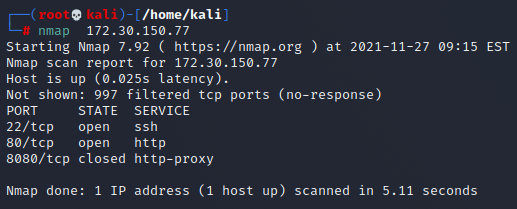
\includegraphics[scale=0.40]{img/nmap.png}}
\section{SQL Injection}
Lorsque nous sommes devant ce type de page de login, une des failles les plus répandue est une faille par injection SQL. Souvent la requête utilisée pour vérifier qu'un login et un mot de passe sont correctes, on envoie ce type de requête à la base de donnée:\newline

\begin{center}
    \textit{SELECT * FROM users WHERE id='\$username' AND passwd='\$password\';}\newline
\end{center}


En entrant dans la case \textit{user} la chaîne de caractère suivante: \textit{admin'--}, la variable \textit{\$username} devient \textit{\$username=admin'--}, on transforme donc la requête SQL précédente:\\




\begin{minipage}{0.4\linewidth}
    \begin{center}
        \textit{SELECT * FROM users WHERE id='admin'--' AND passwd='\$password\';}\newline
    \end{center}
\end{minipage}\hfill
\begin{minipage}{0.40\linewidth}
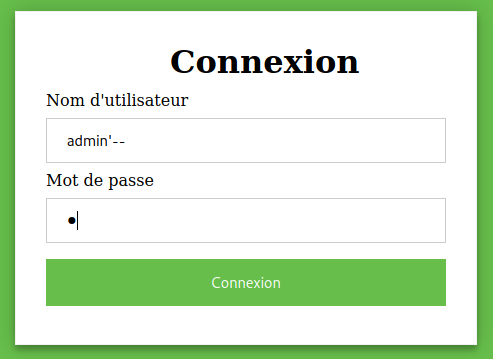
\includegraphics[scale=0.30]{img/login_page.png}
\end{minipage}\\

La partie de la requête après les deux tirets est entièrement ignorée puisqu'elle devient un commentaire. On peut donc entrer n'importe quel mot de passe, si le compte \textit{admin} existe on pourra se connecter. Dans notre cas, cette solution fonctionne et nous sommes redirigés sur une nouvelle page.\newline 


   \centerline{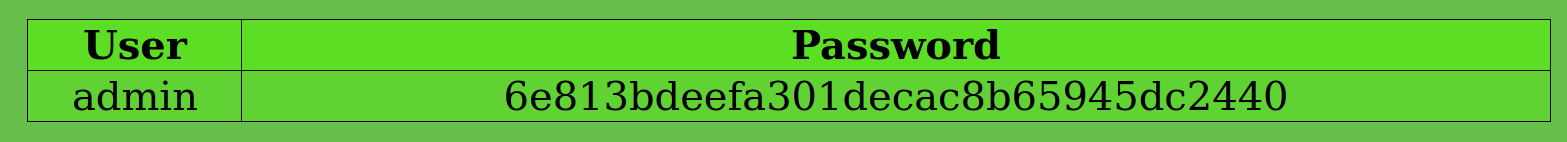
\includegraphics[scale=0.25]{img/hash.png}} 
   \centerline{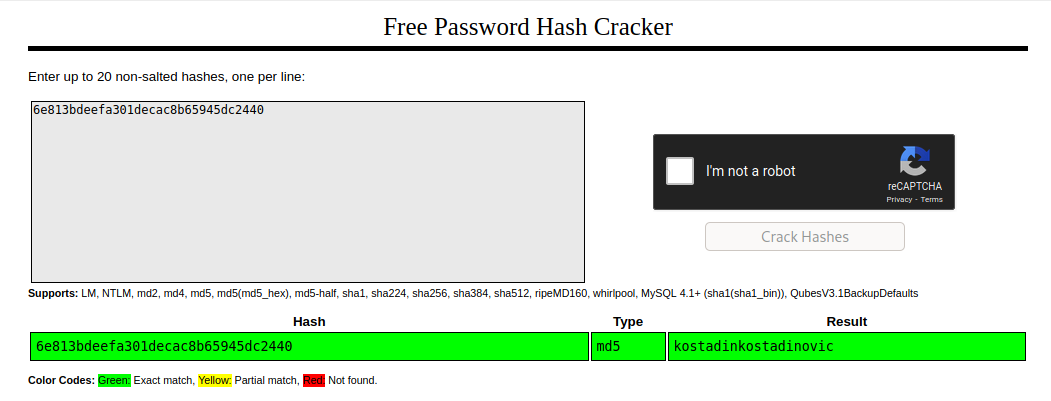
\includegraphics[scale=0.40]{img/password.png}}

Sur cette nouvelle page, nous pouvons voir que nous sommes bien connectés en tant qu'\textit{admin}. Un identifiant ainsi qu'une empreinte md5 sont visibles. On essaie de trouver le mot de passe ayant cette empreinte en allant sur "presque" n'importe quel site proposant ce service. On trouve le mot de passe suivant : \textbf{\hbox{"kostadinkostadinovic"}}. Que pouvons-nous faire avec ce mot de passe ? 

\section{Connexion SSH}
Nous obtenons donc un mot de passe d'un administrateur de ce site web et de la base de données. On se rappelle qu'un port ssh est également ouvert sur la machine. Comme beaucoup de personne, ce serait bête que cette administrateur utilise le même mot de passe pour l'ensemble de ses comptes. Voyons voir, essayons de nous connecter en ssh en tant que root. 

\begin{center}
    \textit{ssh root@ADRESSEIP}\newline
\end{center}

On entre le mot de passe et HOP! miracle, cela fonctionne, nous sommes connectés en tant que root sur la machine.\\

\centerline{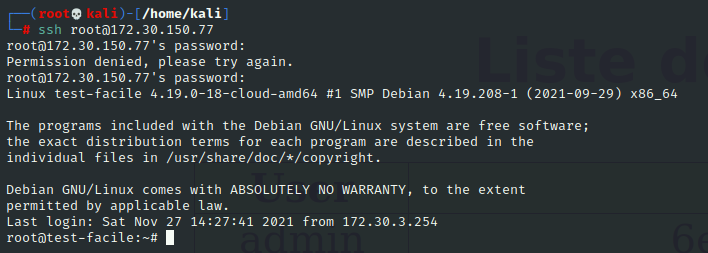
\includegraphics[scale=0.5]{img/ssh_login.png}}

\section{Récupération du flag}
\begin{minipage}{0.55\linewidth}
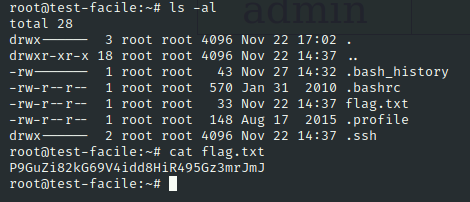
\includegraphics[scale=0.5]{img/flag.png}
\end{minipage}\hfill
\begin{minipage}{0.4\linewidth}
En se baladant rapidement dans les fichiers (notamment le répertoire /root) nous découvrons un fichier nommé \textit{flag.txt}, nous l'ouvrons et nous découvrons le flag du challenge.
\end{minipage}
\end{document}
